
\documentclass{book}
\usepackage{a4,makeidx,fancyheadings}
\usepackage{graphicx}
\usepackage[francais]{babel}
\usepackage[utf8]{inputenc}
\usepackage{fancyvrb}
\usepackage{makeidx}
\usepackage{tabularx}
\usepackage{eurosym}
\usepackage{color}
\usepackage{url}
\usepackage{pdfpages}
\usepackage{xspace}
\usepackage{geometry}
\geometry{ 
      hmargin=3cm,
      vmargin=3cm
}
\usepackage{draftwatermark}
\SetWatermarkText{Provisoire}
\SetWatermarkLightness{0.93}
\SetWatermarkScale{3}



\makeindex
	
\begin{document}
\newcommand{\motcle}[1]{\index{#1}{#1}}
\newcommand{\clecommun}{stockage partagé en réseau\xspace}
\newcommand{\sre}{service relations entreprises\xspace}
\newcommand{\srh}{service ressources humaines\xspace}
\newcommand{\sop}{service organisation et process\xspace}
\newcommand{\scom}{service communication\xspace}
\newcommand{\sconc}{service concours\xspace}
\newcommand{\sintl}{service international\xspace}
\newcommand{\CK}{Christos Karacostas\xspace}
\newcommand{\NB}{Nicolas Beyhurst\xspace}


\thispagestyle{empty}
%-------- fancy headings setting -----------
\rhead[]{}
%\footrulewidth 0.1pt
\rfoot[]{\small\sc S. Genaud}
\pagestyle{fancy}
%------------------------- Page de Garde -------------------
\setlength{\parindent}{0mm}
\setlength{\parskip}{0mm}
\vspace*{\stretch{1}}
\rule{\linewidth}{1mm}
\begin{center}
\Large{Audit du Système d'Information}\\[5mm]
\Large{de l'Ecole de Management de Strasbourg}\\[5mm]
\large{Stéphane Genaud}
\rule{\linewidth}{1mm}
\vspace*{\stretch{2}}
\end{center}
\begin{center}
juin \oldstylenums{2011} \\
\textrm{
$Revision$\\
$Id$\\
$Date$\\
}
\end{center}
%------------------------------------------------------------

\tableofcontents
\newpage


\chapter*{Préambule}

L'EM Strasbourg a connu depuis sa création une croissance exceptionnelle impliquant
le lancement d'un nombre considérable de projets. Un regard est aujourd'hui porté
sur le mode de fonctionnement de l'établissement, et en particulier la façon dont
le système d'information est utilisé pour mener l'activité. C'est l'objet de cet
audit.\\

Ce document a pour objectif de faire l'inventaire des activités des services qui
reposent sur le système d'information. Ce n'est pas une cartographie des processus
mais un témoignage des personnels sur leurs façons de travailler avec un accent
sur les difficultés constatées.\\

Cette état des lieux est effectué à l'occasion d'un changement de direction
(Isabelle Barth succède à Michel Kalika). Il se déroule également à la veille
d'un changement majeur pour l'Université de Strasbourg (UdS) en termes de 
système d'information. L'UdS a défini un nouveau schéma directeur numérique
(SDN) dont la mise en place a déjà amené le remplacement de plusieurs grands
logiciels (e.g SIFAC pour les finances, Moodle comme plateforme pédagogique).
L'essentiel est encore à venir avec la mise en place programmée d'un ERP
(progiciel de gestion intégré) qui permettra de gérer toutes les activités
du c{\oe}ur de métier~: gestion logistique de l'activité pédagogique, des
étudiants et enseignants. C'est le projet \motcle{Alisée}. L'intégration
du système d'information va supprimer d'un coup un grand nombres des
difficultés liées à l'interopérabilité qui sont dérites dans ce rapport.
On peut également attendre de la solution choisie, qui sera dans tous les
cas un logiciel commercial d'un grand éditeur, une ergonomie bien meilleure
que celle des logiciels actuellement déployés.
Le choix du fournisseur est programmé pour la rentrée 2011 et l'échéance
impérative de mise en exploitation est septembre 2013.\\

Bien sûr, cet outil aura un impact considérable sur la manière de travailler
de tous les personnels de l'UdS, et la réflexion actuelle sur le système
d'information de l'EM sera à reconsidérer dans ce nouveau contexte.\\

Néanmoins, les préconisations qui figurent en deuxième partie de ce rapport
portent beaucoup plus sur l'organisation interne des ressources de l'EM
que sur des éléments techniques. A ce titre, elles restent valables
quelque soit les solutions techniques qui seront choisies par l'Université.


 

\chapter{Audit des Services}
 
Les services mentionnés ci-dessous ont été audités entre les 20 et 28 juillet 2011.
L'entretien s'est concentré sur l'identification, pour chaque service, des processus 
principaux et en quoi ils dépendent du système d'information. Pour cahque service,
nous structurons l'audit de la manière suivante~: les processus sont identifiés
(processus fonctionnels), la façon dont les processus fonctionnent actuellement, 
et comment ils s'appuient sur le système d'information est décrite (existant), 
et enfin un jugement glboal est porté sur ces processus (analyse).


\section{Recherche}
\paragraph{Karine Bouvier (KB), Maxime Merli (MM), Thierry Nobre (TN)}

\subsection{Processus fonctionnels}

Le besoin quasi-exclusif est le recensement des publications des chercheurs.
Cette information sert à deux types de processus:
\begin{itemize}
\item[$\bullet$] RC-1) Recenser la production scientifique individuelle ou 
		     collective.
\item[$\bullet$] RC-2) Communiquer sur les thématiques et compétences 
		     en recherche.
\end{itemize}

\bigskip
Pour RC-1, l'information doit être structurée de façon à répondre aux 
exigences des différentes instances d'évaluations (\motcle{AERES}, organismes 
d'accréditation) ou des questionnaires des enquêtes palmarès.
Cette structuration des informations bibliographiques est classique et des
formats existent depuis longtemps (par exemple bibtex). Une spécificité
à prendre en compte est le classement des revues établi annuellement par 
l'AERES.\\

Dans  RC-2, l'objectif est de communiquer vers l'extérieur à travers un 
sites web, un faculty book, etc. Il faut pour cela ré-utiliser les données
factuelles concernant les publications, saisies par les auteurs eux-mêmes
pour RC-1, ainsi que des textes expliquant la structuration de la recherche.\\

D'autres processus peuvent être identifiés, comme par exemple l'organisation
d'une conférence, où la collecte d'information concernant le devenir des
doctorants. Cependant, l'essentiel de ces actions sont ponctuelles et ne 
nécessitent pas un support récurrent du système d'information. La seule 
activité récurrente annexe identifiée est la consultation de l'état des 
finances. Dans ce cas, l'interface web avec \motcle{SIFAC} ainsi que les 
contacts nécessaires avec le gestionnaire des comptes apparaissent satisfaisants.


\subsection{Existant}

L'existant est essentiellement constitué de:
\begin{itemize}
\item la base de données recherche (MS \motcle{Access}), propre à l'EM,
\item l'application, partie de l'\motcle{intranet}, qui gère cette base : 
saisie, modification, consultation de la base.
\end{itemize}
Un premier projet a été mené en 2010 pour construire cette base de données des
publications des enseignants-chercheurs de l'EM Strasbourg. Il a été demandé à 
\CK de développer une fonctionnalité de l'\motcle{intranet} pour cela. L'interface 
de saisie développée n'étant pas assez contrainte, ce premier projet n'a pas 
permis de collecter des données d'une qualité suffisante pour être exploitables
pour produire les statistiques requises (e.g noms de revues orthographiées 
différement). Sur la base de ce constat, l'outil de collecte a été amélioré en 
2011. 

\subsection{Analyse}

Du point de vue des responsables du projet (MM, KB, TN) l'outil donne 
satisfaction en ce qui concerne la qualité des données. Des fonctionnalités 
supplémentaires sont envisagées de manière non urgente (fichier PDF téléchargeable 
de la publication, remontée automatique du papier sur des archives ouvertes comme SSRN%
\footnote{\url{ http://www.ssrn.com/}}).
Il est à noter que l'interface construite ne permet pas de faire d'import (bibtex, 
endnotes,~...), ce qui ne s'est pas révélé être un besoin jusqu'à présent mais
le sera très problement dans le futur. 
La façon dont les informations sont présentées sur les pages web personnelles
des enseignants-chercheurs%
\footnote{\url{http://www.em-strasbourg.eu/enseignants/em-strasbourg-enseignants}}
est également jugé satisfaisant.\\

Les principaux problèmes auxquels ont eu à faire face MM et KB pour la mise 
en place du projet sont:
\begin{itemize}
\item un problème d'interlocuteur : ils n'ont pas trouvé de personne référente
capable de les orienter sur les ressources internes ou externes, ou capable de 
fournir la prestation dont ils avaient besoin.
\item un problème de conduite de projet : une fois la ressource chargée de la 
réalisation identifiée (\CK), leur demande n'a pas fait l'objet d'une conduite
de projet. La planification a été définie de manière imprécise, le cahier des 
charges et les validations peu formalisées.
\end{itemize}



%--------------- Relations Entreprises -----------------------------------

\section{Relations Entreprises et EM Strasbourg Partenaires}

\paragraph{Marie-Hélène Brémont (MHB), Hélène Heintz (HH), Francis Schillio (FS)}
~\\

\textit{Le service Relations Entreprise et Francis Schillio pour 
EM Strasbourg Partenaires ont été audités séparémment mais leurs 
besoins sont confondus. La description est donc regroupée en une 
seule section.}


\subsection{Processus fonctionnels}

Les processus principaux sont:
\begin{itemize}
\item[$\bullet$] RE-1) La recherche ponctuelle d'information sur une entreprise 
			     ou sur un contact professionnel particuliers.
\item[$\bullet$] RE-2) Le filtrage d'un ensemble d'entreprises ou de contacts
			     selon des critères de façon à obtenir un tableau de bord
			     ou envoyer une sollicitation. 
\item[$\bullet$] RE-3) L'enrichissement de la base de données entreprises.
\end{itemize}

\bigskip

L'activité RE-1 permet à FS ou MHB de trouver les coordonnées d'une personne
contact dans une entreprise, d'avoir une vision d'ensemble des personnes 
présentes dans l'entreprise, de voir l'état des cotisations, des versements
effectués, de vérifier à quelles chaires l'entreprise participe, ou toute
information permettant d'avoir une vision globale de l'historique de la 
relation avec cette entreprise.\\

Dans la catégorie RE-2 on trouve le besoin de générer des états récapitulatifs,
comme par exemple lister les entreprises pour lesquelles il y une différence
entre promesse de don et versement réalisés, extraire les entreprises dont 
l'activité est dans tel domaine, etc. Ces actions de filtrage des entreprises
ou des contacts rattachés est également nécessaire pour des actions de 
type publi-postage.\\

L'activité RE-3 consiste à enrichir la base de façon à améliorer les deux
processus précédents. MHB aimerait intégrer les personnes (et leurs entreprises)
participant au concours. L'import des prospects acquis sous une forme quelconque
fait également partie de cette catégorie.
Un point particulier est l'import des diplômés dans cette base. Bien que l'intérêt 
de les y inclure soit évident, l'obsolescence des données est difficile à déterminer.
Seuls les enregistrements des cotisants à jour constituent une information fiable.
Il s'ajoute à cette considération de qualité des données, une difficulté technique
d'identification des entreprises auxquelles ces diplômés doivent être rattachés car
l'entreprise dans la base diplômés n'a pas d'identifiant unique (e.g le numéro SIRET).



\subsection{Existant}

Bernadette Fischbach travaille avec un outil développé en 2001 par 
une étudiante (Cécile Henner) du PGE IECS. L'outil est une base 
\motcle{Access} interfacée. La base comporte de l'ordre de 10000 fiches 
entreprises dont environ 2000 réellement actives. La qualité
des données est maintenue par le travail quotidien de Bernadette
Fischbach. De plus, une opération d'ajout et de vérification des
numéros SIRET a été confié à un prestataire extérieur (environ
60-70\% des entreprises ont été ``SIRETé'').\\

En septembre 2010, la direction de l'EM (Michel Kalika) a confié
à l'auteur de cet audit une mission pour mettre en place un véritable
\motcle{CRM}. Cette demande émanait du service relation entreprise (Francis 
Schillio). Il a été décidé d'acheter cette prestation et de ne rien 
développer en interne étant donné la charge de travail de Christos 
Karacostas. Le calendrier initial prévoyait une mise en production 
à la fin du printemps 2011. A la demande du service relations 
entreprises, le calendrier du projet a été reporté pour une mise en 
production fin 2011.
Le cahier des charges après étude de marché et audition de
plusieurs offres a été établi d'après l'expression des besoins
centrée autour du service relations entreprises, stages et apprentis.
Ce cahier des charges, base de l'appel d'offre figure en 
annexe~\ref{ch:annexe-crm}.\\

\begin{figure}[hbt]
\begin{center}
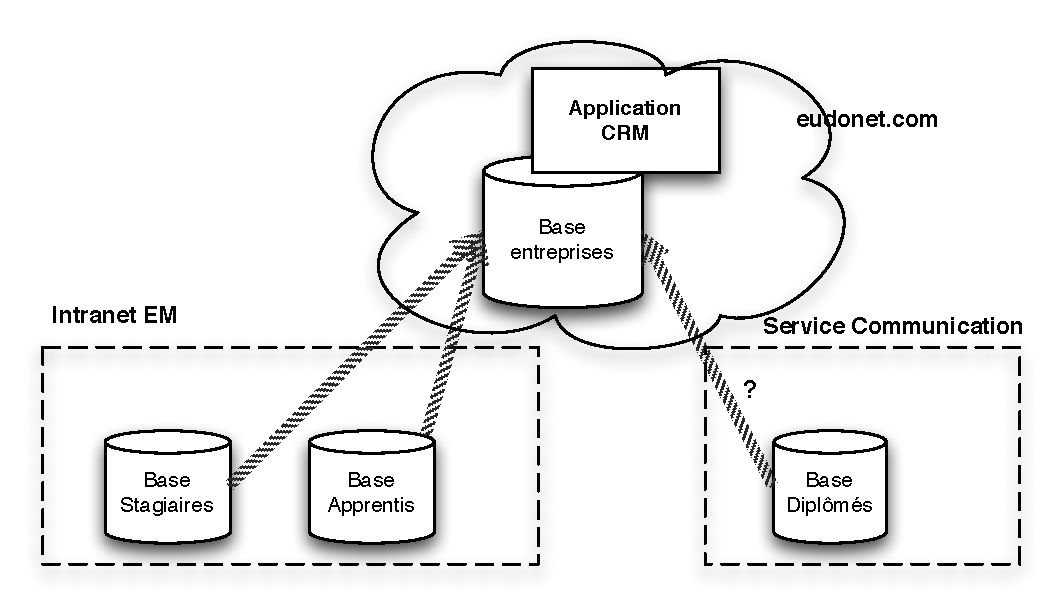
\includegraphics[width=.9\linewidth]{figs/crm_overview.pdf}
\end{center}
\caption{Positionnement du \motcle{CRM} dans le système d'information de l'EM}
\label{fg:crm_overview}
\end{figure}

Le périmètre du \motcle{CRM}  a été volontairement limité au \sre. L'analyse 
des besoins a montré que le \motcle{CRM} ne pouvait pas prendre en charge 
toutes les fonctionnalités de gestion des stages et de l'apprentissage. 
Ceci nécessiterait d'en faire un outil de gestion de scolarité également
(par exemple mémorisation des notes de stage). Comme le montre la 
figure~\ref{fg:crm_overview}, il a été décidé que la liste des étudiants 
en stage et apprentissage serait régulièrement exportée (fréquence 
mensuelle environ) vers le \motcle{CRM} afin de l'enrichir.\\

Etant donné que cet outil est un produit commercial dont le coût est
proportionnel au nombre de licences utilisateurs achetées, et qu'il
donne des informations financières sensibles sur les versements des
entreprises, cet outil reste confiné au \sre. D'autres services, comme
les scolarités, pourront profiter de cet outil indirectement en adressant
des requêtes au \sre.

\subsection{Analyse}
Le \sre travaille depuis dix ans avec une base de données qui lui est
propre. Cet outil est bien maîtrisé par Bernadette Fischbach qui en
a une longue expérience et possède une connaissance profonde des 
entreprises avec lesquelles l'EM a des relations régulières. \\

Cet outil est cependant limité de par sa conception et ses connexions
avec les autres bases de données du S.I. Sa conception rend l'extraction
de données assez difficile car des requêtes spécifiques nécessitent 
l'intervention de \CK. La base de données entreprises est autonome, ce
qui explique la longévité du système, mais s'avère limitante aujourd'hui.
Le nouveau projet \motcle{CRM} doit améliorer cette situation. D'une part, l'outil
sera multi-utilisateurs, accessible en ligne (il est prévu qu'il soit 
consultable de l'antenne Parisienne), permettra à chaque utilisateur de 
construire ses reqûetes à travers son interface, et sera paramétrable. 
D'autre part, des données externes (stagiaires et apprentis, prospectivement 
données du concours et diplômés) seront importées pour enrichir la base.\\

Ce projet \motcle{CRM}, qui ne peut s'insérer complètement dans le S.I. global
(car il faudrait y gérer aussi la scolarité) est destiné au moyen terme,
en attendant d'analyser le produit \motcle{CRM} qui sera adopté dans le schéma
numérique directeur de l'UdS (probablement disponible à l'horizon 2014). 

  

%---------------  Communication  -----------------------------------
\section{Service communication}

\paragraph{Michèle Schmidt (MS), Isabelle Suhr (IS), Marine Julien (MJ), 
\NB (NB), Thomas Arbib (TA).}

\subsection{Processus fonctionnels}
Les processus nécessitant le support du système d'information peuvent 
être rangés en quatre catégories:
\begin{itemize}
\item[$\bullet$] CO-1) La communication d'informations à des publics ciblés.
\item[$\bullet$] CO-2) La gestion technique d'évènementiels.
\item[$\bullet$] CO-3) La collecte d'informations pour répondre aux enquêtes de type 
      palmarès.
\item[$\bullet$] CO-4) L'analyse de l'attractivité de chaque formation académique.
\end{itemize}
\bigskip

Dans la catégorie CO-1 le besoin est de constuire des \textbf{listes 
pertinentes et ciblées d'adresses electroniques}. La difficulté
est bien sûr différente selon que la communication est à destination
d'un public interne ou externe à l'établissement.

En interne, il est nécessaire de disposer d'un \textbf{annuaire}
fiable et précis du personnel et des étudiants. 

Pour la communication vers l'extérieur, le mailing est souvent 
fait de manière indirecte : l'information à communiquer transite par
le service en charge du public visé, avec un contrôle informel des 
destinataires par le service en question. Ainsi, une invitation à un 
colloque académique sera transmise par Karine Bouvier (Recherche),
une invitation à un carrefour métier sera transmise par Bernadette 
Fischbach (Relations Entreprises) ou une information aux étudiants
est transmise à la scolarité concernée pour redifusion. La communication 
vers l'extérieur nécessite donc une \textbf{base de prospects} fiable 
qui puisse être consolidée avec les données d'autres services (scolarité, 
relation entreprises, recherche), ainsi que des \textbf{procédures 
de collectes} de nouveaux prospects le plus automatisées possibles.\\

Dans la catégorie CO-2 on trouve en particulier l'activité de création
de mini-sites web par NB permettant de gérer chaque évènement (inscriptions,
programmes, informations pratiques, etc) ou du site des diplômés (alumnis).
Cette activité ne dépend pas du système d'information excepté pour
la mise à jour de l'annuaire des diplômés. Elle est au contraire 
support à la catégorie CO-1 en fournissant les données déposées par les
visiteurs sur les sites web.\\ 

La catégorie CO-3 nécessite de rassembler des statistiques provenant de 
nombreuses sources. Les informations à collecter et les services qui les 
produisent sont présentés en figure~\ref{fg:comm_flux}.
\begin{figure}[hbt]
\begin{center}
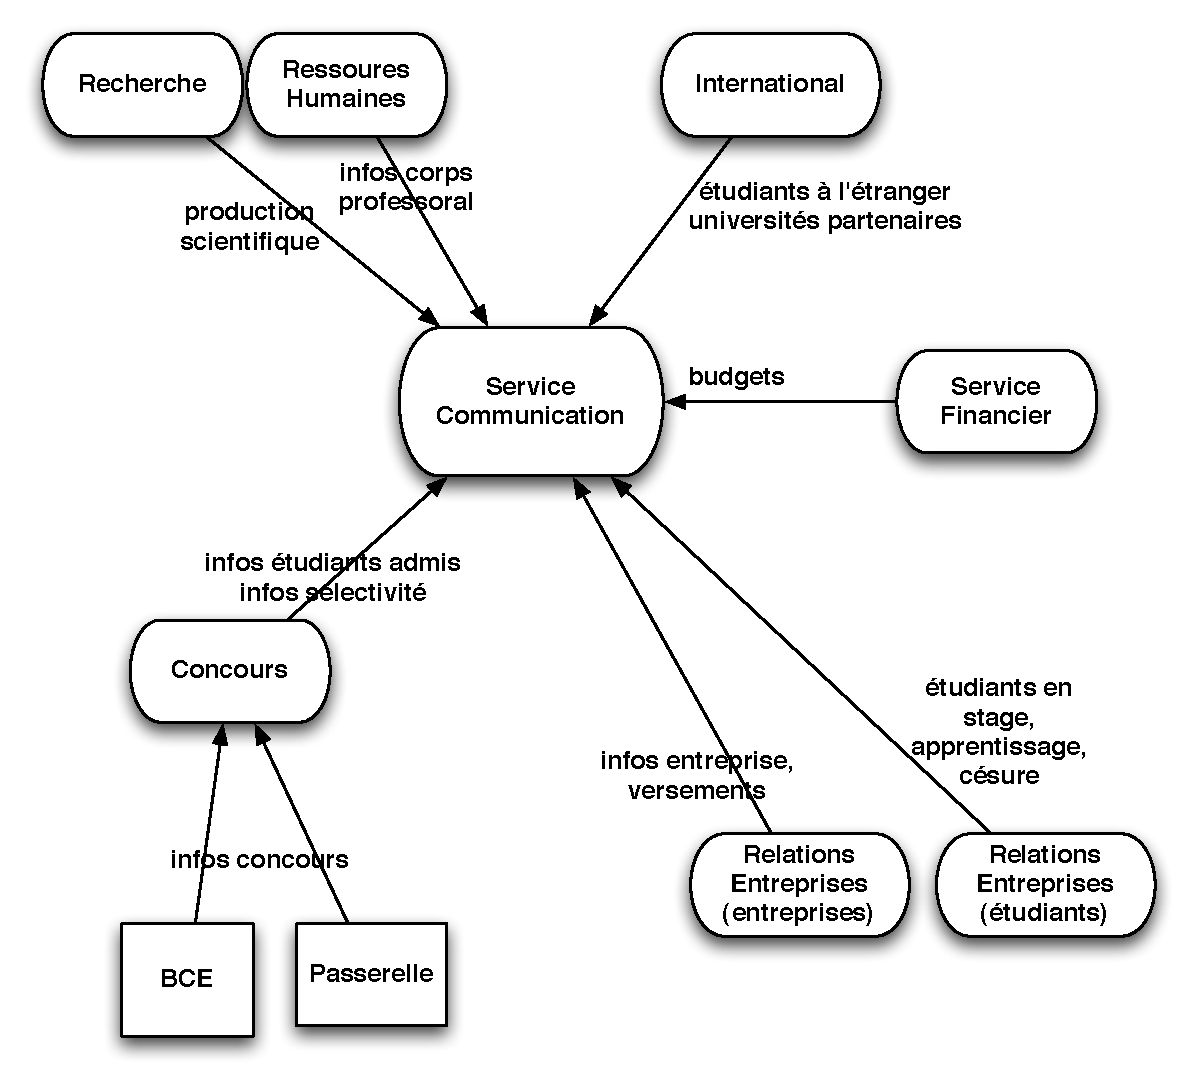
\includegraphics[width=.75\linewidth]{figs/comm_flux.pdf}
\end{center}
\caption{Les flux d'informations nécessaires pour répondre aux enquêtes de 
type palmarès}
\label{fg:comm_flux}
\end{figure}
Dans ces enquêtes, MS sépare les différentes questions posées et délègue
dans les services appropriés la charge de trouver l'information.\\


Dans la catégorie CO-4, on compte les deux enquêtes intégrés (PGE et Master 
Universitaires, formation continue) qui apportent de l'information sur la 
typologie des étudiants nouvellement recrutés et la façon dont ils ont eu 
connaissance de l'établissement et de la formation. Cette information permet 
au service de mieux comprendre l'impact des différents supports de 
communication.

Rentre également dans cette catégorie les statistiques sur les formations
Master et EE à tous les stades du recrutement. IS a construit au cours 
des années un historique de ces statistiques, formation par formation,
et peut ainsi mieux analyser l'attractivité de chacune des formations.
Ces données permettent aussi d'ajuster les opérations de communication.
Par exemple, un nombre plus faible de demandes de dossier d'inscription 
à une formation peut suggérer une opération de communication ciblée.
Pour collecter ces statistiques, une synthèse des données était auparavant
demandée via fichier partagé en réseau (à travers l'espace de stockage nommé
\textit{commun}\index{\clecommun}), à la scolarité aux différents étapes 
du recrutement (nombre de dossiers demandés, dossiers reçus, dossiers acceptés). 
L'accroissement du nombre de formations et la mise en place d'ARIA rend 
cette procédure caduque. Aujourd'hui, ces données dont récupérées
directement d'ARIA mais la précision est plus faible et \motcle{Aria} ne 
conserve que les pré-inscriptions pour l'année en cours. Il faudrait
donc disposer d'un stockage auxiliaire pour fabriquer un historique.


\subsection{Existant}
\begin{itemize}
\item Pour les processus de catégorie CO-1 concernant la communication interne
	les données d'annuaire fournies par l'\motcle{intranet} EM %
	\footnote{\url{http://intranet.em-strasbourg.eu/adm/fr/grh/coordonnees.html}}
	sont utilisées de manière efficace pour communiquer par mail.
	En revanche, il n'existe pas d'annuaire plus complet permettant
	par exemple de connaître les fonctions et les status (problème 
	d'édition des cartes de visites en français et anglais).


	Pour CO-1 concernant la communication externe,
	il existe des fichiers prospects dispersés et conservés dans des 
	formats techniques de stockage différents. Le tableau en figure 
	\ref{fg:comm_prospects} liste ces différents fichiers.
	L'utilisation de fichiers \motcle{Excel} est la plus courante et considérée 
	la plus pratique actuellement.

\begin{figure}[hbt]
\begin{center}
	\begin{tabular}{llll}
	\hline
	\hline
	public	& source	 & format de stockage \\
	\hline
	prospects par évènements & inscription sur  mini-sites &  base de données, export csv (\motcle{Excel})\\
	prospects formation continue  & pré-inscriptions ARIA & import csv \\
	prospects diplômés      & service diplômés &  import csv, puis base de \\
					&			 &  données gérée dans le service Comm. \\
	étudiants après CRD 	& données \motcle{Apogée} & import csv \\
	journalistes 		& contact personnel	& carnets d'adresse \\
	salons, contacts divers	& contact mail, carte visite & carnets d'adresse, fichiers \motcle{Excel}\\ 
	VIP institutionnels	& contact mail, carte visite & carnets d'adresse, fichiers \motcle{Excel}\\ 
	\hline
	\hline
	\end{tabular}
\end{center}
\caption{Fichiers prospects utilisés pour communiquer vers l'extérieur, source 
	d'acquisition et format de stockage}
\label{fg:comm_prospects}
\end{figure}
	Ceux-ci  ont pu être constitués par la collecte des informations saisies 
	par un participantà un évènement (inscription sur mini-site), ou lors de 
      salons (saisie manuelle). L'application ARIA de pré-candidature 
	(application de l'UdS) peut aussi être utilisée pour produire des 
	fichiers prospects (personnes ayant entamé une démarche d'inscription 
	sans finaliser).

\item Dans la catégorie SC-2, NB développe de manière réactive des sites couplés 
	à des base de données selon des formats ouverts (logiciels libres \motcle{PHP}, 
	\motcle{MySQL}) qui répondent aux besoins ponctuels de gestion d'un évènement, 
	permettant de conserver de manière pérenne ces données. Son action est 
	cependant intrinsèquement limitée par la difficile connexion à d'autres 
	sources d'informations (\motcle{intranet} EM et applications du S.I. UdS).

\item Dans la catégorie SC-3 les données ne sont pas stockées mais simplement 
	reportées aux demandeurs dans le format souhaité.

\item Dans la catégorie SC-4 les processus sont manuels et les données 
	enregistrées dans des fichiers personnels.
\end{itemize}



\subsection{Analyse}

D'une part, le \scom a globalement besoin d'informations réparties dans la 
quasi-totalité des applications du système d'information. Aujourd'hui, la 
collecte des informations nécessaires est déléguée aux services les plus 
proches de ces applications. Cependant, il est probable que ce fonctionnement 
resterait recommandable même si le système d'information était directement 
interrogeable par le \scom, car les services qui possèdent les données
souhaitent en contrôler l'utilisation.\\

D'autre part, le \scom possède et produit ses propres données, principalement 
des contacts. La gestion de ces données est hétéroclite en raison des supports 
divers. La disponibilité de l'information n'est pas totalement maîtrisée car 
certaines données peuvent échapper aux sauvegardes car non entreposées dans des 
espaces de stockage sauvegardés par les services informatiques. Les outils 
bureautiques utilisés font que l'information est peu efficiente et peu efficace.\\


Du point de vue des applications, la présence d'un informaticien au sein du 
service aide considérablement à la résolution de problèmes techniques ponctuels. 
Ceci ne peut cependant pas remplacer la mise en place se solutions applicatives 
plus globales. Il manque en particulier un outil pour faire du mailing de masse 
compatible avec les règles de sécurité anti-spam de l'UdS. L'emploi d'outils 
collaboratifs adaptés permettrait également de gagner en efficacité. 

	

%------------------------ R H -------------------------------------------------

\section{Service Ressources Humaines}

\paragraph{Laurie Walbrou (LW), Emilie Kaës (EK)}


\subsection{Processus fonctionnels}
\label{sc:rh-process}
Les processus nécessitant le support du système d'information peuvent 
être rangés en deux catégories:
\begin{itemize}
\item[$\bullet$] RH-1) La gestion du personnel administratif et enseignant
\item[$\bullet$] RH-2) L'organisation d'évènements
\end{itemize}
\bigskip

La catégorie RH-1) représente l'immense majorité de l'activité.

Le besoin est de \textbf{collecter des informations pertinentes
sur le personnel} de l'EM. La pertinence se décline selon
deux besoins plus spécifiques:
\begin{itemize}
\item RH-1.1) les besoins pour répondre aux accréditations, enquêtes 
	palmarès, au label diversité, écrire le bilan social.
\item RH-1.2) les besoins issus du dialogue de gestion avec l'Université.
\end{itemize}

\bigskip

Le besoin RH-1.1 nécessite des informations très nombreuses, précises
et changeantes d'années en années. Ainsi l'accréditation AACSB demande
par exemple pour chaque enseignant combien d'années il a passé à l'étranger 
les cinq dernières années. Ces contraintes spécifiques obligent 
l'établissement à posséder une base propre de ces informations étant donné 
que les logiciels de gestion de RH disponibles à l'UdS ne peuvent pas 
cas fournir d'informations aussi spécifiques. Il est probable que cette
contrainte perdure après la mise en place du futur SI RH du schéma numérique
directeur de l'UdS (horizon 2014), à moins que celui-ci ne soit extrêmement 
paramétrable et qu'un support important de la part de l'UdS soit consacré 
aux demandes spécifiques.\\

Le besoin RH-1.2 est beaucoup moins exigeant. Il fait appel à toutes
les informations administratives contenues dans \motcle{Harpege} 
et \motcle{SOSIE} concernant les personnels.\\


Concernant les activités de la catégorie RH-2 le besoin exprimé 
est la mise en place d'un agenda partagé permettant d'éviter
les conflits de date lors d'organisations d'évènements, et de 
diffuser l'information évenementielle sans faire d'invitation
par mail mais par un mécanisme de publication/souscription
(e.g fil RSS, synchronisation d'agenda).  



\subsection{Existant}

Le processus correspondant au besoin RH-1.1 a conduit à mettre en
place une procédure pour le recrutement des vacataires. Cette procédure
est décrite par le diagramme de séquence en figure \ref{fg:rh_seq_vacataires}.
Elle vise à enregistrer les informations perinentes concernant les enseignants
au moment de la candidature en analysant le CV d'un candidat retenu. Ces
informations sont enregistrées dans un fichier \motcle{Excel} maintenu par EK.

\begin{figure}[hbt]
\begin{center}
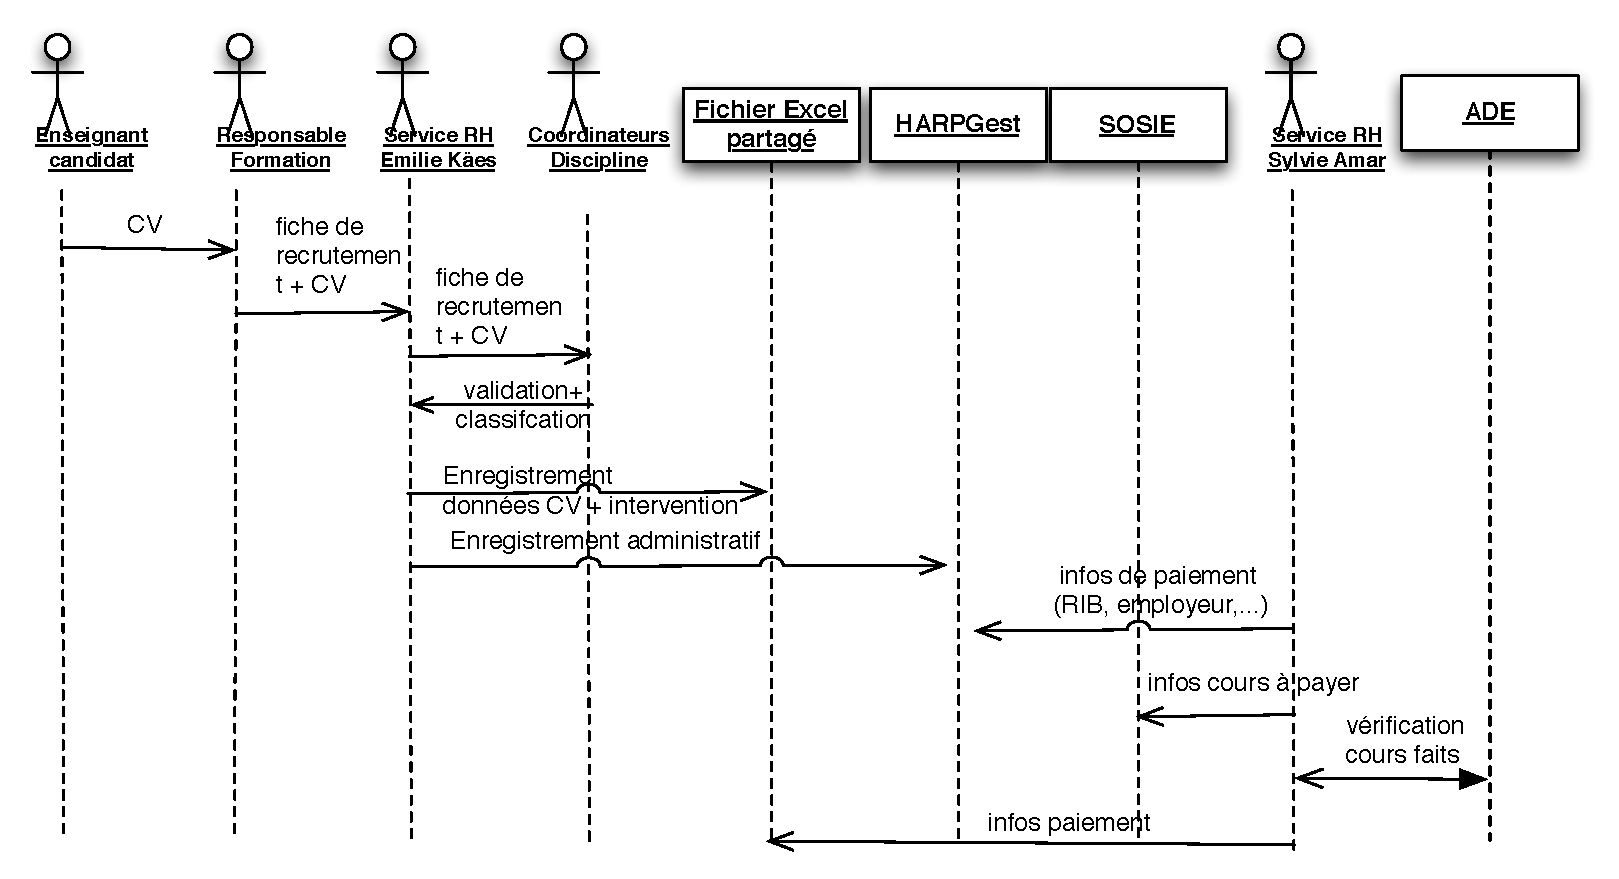
\includegraphics[width=\linewidth]{figs/rh_seq_vacataires.pdf}
\end{center}
\caption{Diagramme UML de séquence pour la procédure d'enregistrement d'un vacataire.}
\label{fg:rh_seq_vacataires}
\end{figure}

Le reste de la procédure vise à enregistrer administrativement l'enseignant
dans le S.I. de l'UdS: application \motcle{SOSIE} pour les heures effectuées 
et payées et application HARPGest pour mémoriser les informations d'état civil 
et celles nécessaire au paiement des heures. 
Cependant, ces \textbf{applications se révèlent totalement inefficaces} dans 
le reste du processus. Ainsi, les extractions d'\motcle{HARPGest} ne peuvent 
fournir que les noms, date de naissance et nationalité d'une personne. 
\motcle{SOSIE} ne liste que les heures de cours pouvant donner lieu à rétribution
et sur des intitulés de matière qui peuvent avoir changé dans \motcle{Apogée}.
Pour connaître l'état des paiements des heures, la procédure en place prévoit
que Sylvie Amar édite le fichier Excel (\index{\clecommun} partagé en réseau) 
pour y inscrire les heures payées pour chaque enseignant.\\

Les processus de la catégorie RH-1.2 subissent les mêmes manquements en terme
de support du système d'information. Le dialogue de gestion annuel implique
de faire à minima un état des lieux précis des personnels permanents de 
l'établissement. Cependant, les applications en place ne permettent même pas
d'obtenir les numéros de postes sur lesquels les personnes sont en place.
LW maintient son propre fichier pour ces postes. Elle obtient cette information
par contact téléphonique auprès d'une responsable au service RH de l'UdS, et
non sur la base d'une importation automatique de données.\\

Concernant le besoin RH-2, aucun outil n'est aujourd'hui en place.

\subsection{Analyse}
\label{sc:rh-analyse}
Le support du S.I. aux RH est en train d'évoluer. Avant la mise en place
de la procédure décrite (figure~\ref{fg:rh_seq_vacataires}), et relativement 
aux processus décrits ici, le service RH fonctionnait sans aucun support réel 
du point de vue des systèmes d'information. La perspective de créer un outil 
spécifique pour gérer les candidatures et CV a été évoquée dès 2006 mais ne 
s'est pas réalisée. 
Confrontés aux demandes des accréditations, depuis 2010, les \srh et
Organisation et Process ont passé de l'ordre de 10 mois hommes pour analyser 
les CV papiers des enseignants intervenant (de l'ordre de 500 intervenant). 
Un nouveau projet a été conçu, intitulé \textit{Base de données CV}, dont 
le document de travail est copié en annexe~\ref{ch:rh-cvtheque}.
Idéalement, ce projet devrait mis en production en décembre 2011. 
Cependant, le manque général de planification des projets et la faible 
formalisation du cahier des charges pourrait rendre cette échéance improbable.\\

La procédure actuelle est adaptée aux demandes et devrait permettre de 
répondre assez efficacement aux questions. Cependant, le fichier \motcle{Excel}
dans lequel figure quasiment toutes les données est le point névralgique
de ce processus, et à ce titre représente un risque certain. Etant sur
un espace commun, il sauvegardé%
\footnote{Sauvergarde de cet espace de stockage géré par la direction 
informatique de l'UdS selon \CK.
}
mais la gestion des droits étant difficile, on peut imaginer qu'un autre 
administratif corrompe (intentionnellement ou non) les données y figurant.\\

Concernant les applications, il faut retenir que les applications
du S.I. de l'Université ne fournissent quasiment aucune information en
retour (\motcle{SOSIE} et \motcle{HARPGest}). L'\motcle{ADE} permet de 
vérifier les heures de cours effectuées. L'\motcle{intranet} EM n'est pas 
du tout utilisé par le service RH.
 



% --------------- A C C R E D I T A T I O N S ----------------------
\section{Service Organisation et Process}

\paragraph{Fatiha Bouterâa (FB), Maxime Merli (MM)} 
~\\

\textit{Pour l'audit dans ce service, le sujet prioritaire concerne les 
accréditations, d'où la présence de MM pour l'entretien. Cependant, pour 
garder la cohérence du document, cette section reprend les besoins du service.}

\subsection{Processus fonctionnels}
\label{sc:sop-process}

Une très grosse partie de l'activité du service est aujourd'hui en rapport 
avec les accréditations. 
\begin{itemize}
\item[$\bullet$] OP-1) La production de statistiques pour répondre aux 
			     accréditations.
\item[$\bullet$] OP-2) Le criblage du contenu pédagogique pour répondre 
			     aux accréditations.
\end{itemize}
La gestion de la qualité est une autre activité que le SI peut contribuer à
améliorer, notamment à travers le processus suivant:
\begin{itemize}
\item[$\bullet$] OP-3) La gestion des fiches d'amélioration.
\end{itemize}
\bigskip
Les activités pour OP-1 se décomposent selon les flux d'information 
nécessaires au document à produire (différents pour chaque accréditation). 
Les flux sont comparables à ceux sollicités par le \scom. Ils sont présentés 
en figure~\ref{fg:accred_flux}.
\begin{figure}[hbt]
\begin{center}
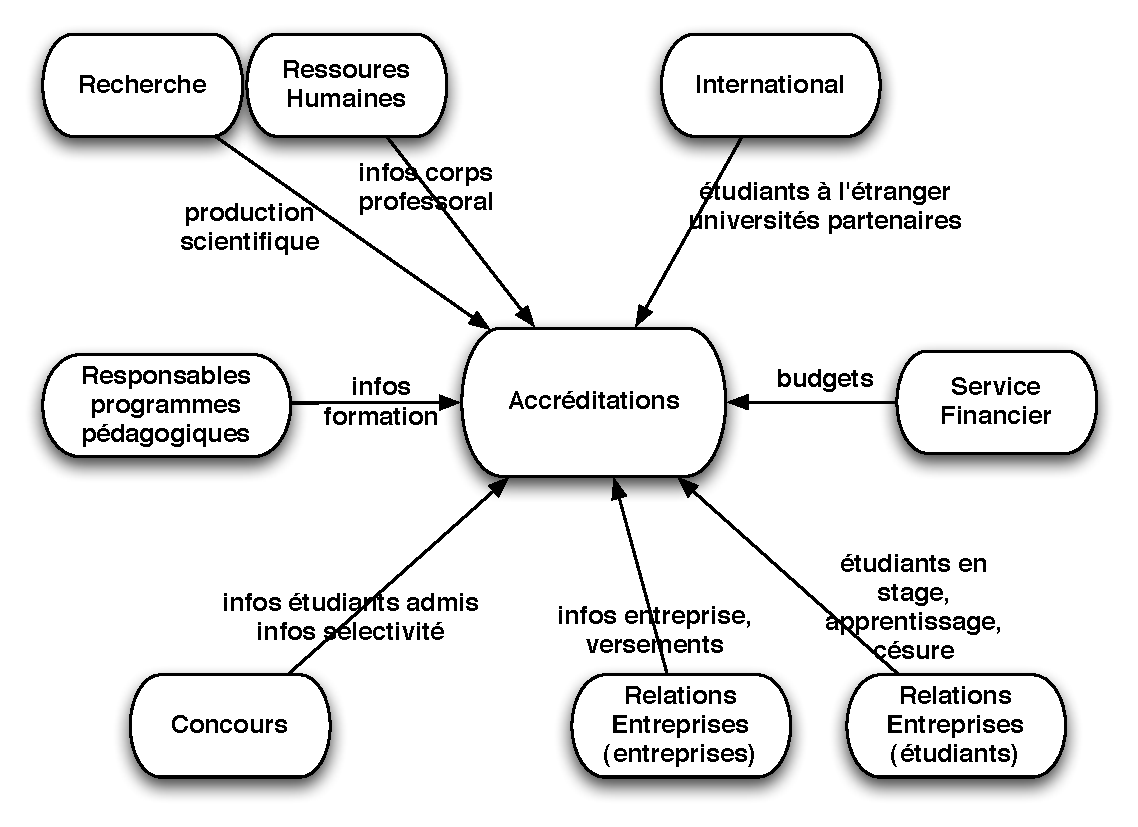
\includegraphics[width=.75\linewidth]{figs/accred_flux.pdf}
\end{center}
\caption{Les flux d'informations nécessaires pour les accréditations}
\label{fg:accred_flux}
\end{figure}
En plus des informations que le \scom doit aggréger, le \sop doit obtenir des 
données précises sur les programmes pédagogiques. Bien que cohérentes ces 
informations nécessitent de les demander à plusieurs sources: par exemple
le nom des diplômes, des listes d'étudiants inscrits, les volumes horaires,
seront obtenus via les scolarités et la base de l'intranet EM (intervention de 
\CK), les taux de sélectivité à l'entrée des formations seront obtenus du \sconc 
pour le PGE ou des responsables de formation pour les autres formations, 
tandis que l'année de création d'une formation nécessite
de faire une recherche auprès du créateur de la formation (la mémoire n'étant
pas infaillible, un recours à des documents annexes comme les plaquettes peut
être nécessaire).
Une difficulté supplémentaire s'ajoute du fait des questions posées qui 
impliquent souvent un \textbf{historique} sur les 3 à 5 dernières années, comme 
par exemple nombre de diplômés sur les trois dernières années.

Obtenir ces données se révèle encore plus compliqué pour les diplômes hébergés
hors Strasbourg (Maroc, Nancy, Paris).\\


L'activité OP-2 concerne la gestion de l'\emph{Assurance of Learning} (AOL).
Un document d'accréditation AACSB implique, outre les données quantitatives,
d'être capable de présenter une maquette pédagogique en conformité avec des
objectifs pédagogiques (\emph{learning goals}) définis au préalable. 
Les besoins sont ici de pouvoir extraire automatiquement des vues matricielles
de synthèse sur l'ensemble des formations. Cela peut être des tableaux montrant
quels \emph{learning goals} sont satisfaits par quels cours. 
En plus de ces indicateurs de la cohérence de la proposition pédagogique, il
faut pouvoir mettre en place des indicateurs sur l'efficacité de la formation,
c'est-à-dire définir des critères de réussite formulés pour chaque formation
et mesurer les taux de réussite et les taux d'atteinte des objectifs
pédagogiques.

L'évaluation des enseignements est également nécessaire dans ce processus.

Ces activités OP-2, qui agissent sur la présentation structurée des 
programmes pédagogiques, sont menées en étroite collaboration avec les directeurs
délégués des programmes dans leur activité PP-2, qui agit elle sur le contenu
même de la formation (voir section~\ref{sc:pp-process}, page~\pageref{sc:pp-process}).
\\

L'activité OP-3 devrait être collaborative, et ouverte aux utilisateurs à 
travers une interface web. Une fiche d'amélioration devrait pouvoir
être suivie en temps réel: personne en charge du dysfonctionnement constaté, 
statut de la résolution du dysfonctionnement (en cours, traité), et son 
efficacité testée après résolution (délai programmé après 
lequel le test d'efficacité est fait). Un système de relance automatique
par mail doit y être adjoint pour s'assurer de l'avancement des traitements.



\subsection{Existant}

Le processus OP-1 contient le processus RH-1.1 décrit précédemment dans la 
section~\ref{sc:rh-process} (partie qui concerne les renseignements sur les
personnels enseignants et administratifs). Comme pour RH-1.1., le même constat 
s'applique pour toutes les autres données à collecter: le S.I. ne permettait pas 
d'obtenir ces données initialement et des fichiers ad-hoc ont été construits quand 
il a fallu produire le rapport la première fois. Ces fichiers sont aujourd'hui vitaux pour
rédiger les dossiers d'accréditations à venir.\\

Pour OP-2 la gestion de l'AOL peut utiliser l'\motcle{intranet} de l'EM qui
permet à chaque enseignant de saisir les données relatives à chacun de ses 
cours\footnote{Exemple: \url{http://tinyurl.com/3ek7rus}}. Ces données 
constituent une base précieuse pour le travail de structuration de l'ensemble
de la maquette. De nouvelles fonctions pourraient aussi être ajoutées facilement
en cas d'urgence.\\

Concernant OP-2 également, une procédure d'évaluation existe depuis une dizaine 
d'années dans le programme PGE et a été généralisée à tous les programmes. Elle 
propose aux étudiants d'évaluer anonymement chaque cours auquel il était inscrit. 
Cette procédure utilise exclusivement l'\motcle{intranet} EM.
L'évaluation de la formation dans sa globalité est proposé par un autre service à l'UdS%
\footnote{\url{http://sondages.unistra.fr}, (logiciel limesurvey)}.\\

Pour OP-3 seul un support sous forme d'un fichier \motcle{Excel} non partagé (possédé par Angèle 
N'zinga) existe actuellement. Cependant, le besoin est
bien connu dans le monde du logiciel et de nombreux outils existent%
\footnote{\url{http://tinyurl.com/3eyvb4y}}
et pourraient être transposés ici.


\subsection{Analyse}
\label{sc:sop-analyse}

Dans son travail sur les dossiers d'accréditation, le \sop et les autres
personnels impliqués ont effectué un travail considérable pour produire
les informations quantitatives exigées par ces dossiers. Ces procédures
de collectes d'information sont très faiblement automatisées. Les données
les plus facilement exploitables sont celles provenant de l'\motcle{intranet}
ou que l'EM contrôle : base entreprises, stages, apprentis, concours. 
L'exploitation des données nécessite quand même l'intervention de \CK. 
Pour les données qui étaient hors de ce champ, le \sop a enregistré de
nombreuses informations dans des fichiers à part, avec les mêmes risques
que ceux mentionés précédemment (e.g section \ref{sc:rh-analyse}). 
Il serait donc judicieux de ré-injecter toutes ces informations dans le S.I.
global mais ceci implique des développements conséquents dans l'intranet.\\


L'AOL pourrait faire l'objet d'un projet démarrant immédiatement dans
l'objectif d'une accréditation AACSB à l'automne 2014. Il est en effet 
nécessaire de déployer le processus pendant deux à trois ans (durée
d'un cycle de formation pour un étudiant), car l'accréditation impose de
présenter les résultats obtenus sur au moins un cycle. Le démarrage de
l'exploitation devrait dans ce cas démarrer au premier semestre 2012,
ce qui impliquerait une défintion des besoins et une réalisation logicielle
à l'automne 2011.

Le S.I. devrait alors être repensé pour recueillir puis formatter les 
données décrites précédemment. Il devrait également prendre en compte 
les possibilités qui seront offertes par le futur S.I. \motcle{Alisée} 
de l'UdS. Etant donné que ces questions sont transversales à toutes les 
formations, concevoir un modèle de données capable de s'adapter à la 
variabilité des angles de vues, et capable de s'articuler avec les 
enseignants est un projet complexe qui nécessite, après une mise en 
{\oe}uvre rapide, une phase d'ajustement assez longue, probablement sur
plusieurs semestres. 




% --------------- C O N C O U R S ----------------------

\section{Service concours }
\paragraph{Aida Saïd (AS)}
~\\

\subsection{Processus fonctionnels}
\label{sc:concours-process}

\begin{itemize}
\item[$\bullet$] CC-1) Faire la promotion du concours
\item[$\bullet$] CC-2) Organiser le concours
\item[$\bullet$] CC-3) Produire les résultats du concours
\end{itemize}
\bigskip

CC-1 concerne la centralisation des informations revenant des
opérations de promotion: promotion par des étudiants auprès  des 
élèves en classe préparatoire, salon, et journées portes 
ouvertes.\\ 

CC-2 est l'activité d'organisation comprend deux phases. Il 
faut d'abord solliciter des personnes du monde professionnel 
ou académique à devenir membre de jury. Il faut ensuite gérer
la planification des jurys d'après les informations de
disponibilité des candidats, transmises quotidiennement
par les organisations Passerelle et BCE.\\

CC-3 consiste en la saisie des notes des jurys dans un fichier
\motcle{Excel} (double saisie pour éviter les erreurs). Ce fichier est 
envoyé à Passerelle, resaisi sur un site web dans le cas de BCE.
En retour, AS obtient le rang et la moyenne des candidats sous
la forme d'un fichier \motcle{Excel}. L'EM décide de la barre d'admissibilité
et la communique à Passerelle et BCE. Ces derniers peuvent alors
communiquer les listes d'admissions.

A partir de septembre, il faut produire des statistiques sur le
résultat du concours, qui seront utilisées par plusieurs services.


\subsection{Existant}
CC-1) 
La collecte tout au long de l'année de prospects étudiants
ne donne pas lieu à un traitement rationel de l'information.
Les compte-rendus faits par les étudiants après les visites de
promotion en classes préparatoires sont des documents papiers
archivés mais inexploités. Occasionnellement, AS saisit dans un
fichier \motcle{Excel} des noms et adresses de prospects étudiants ayant 
manifesté un intérêt pour l'EM lors de salons ou journées portes 
ouvertes. La source la plus abondante pour des contacts reste
les fichiers de BCE et Passerelles, mais ces personnes ne restent
prospects qu'un laps de temps assez court.\\


CC-2)
La sollicitation s'est faite cette année en compilant des
fichiers d'adresse provenant de plusieurs sources: contacts
EM Strasbourg Partenaires, diplômés, entreprises versant la
taxe d'apprentissage, enseignants vacataires inscrits dans
l'intranet et anciens membres de jury. Ces contacts ont été
invités par mail à s'inscrire sur un site web%
\footnote{\url{http://aestirh.em-strasbourg.eu/jurys}}
construit et géré par le \scom (\NB).
Cette procédure qui vient juste de remplacer une procédure
``papier'' est tout à fait adaptée au besoin. Elle va permettre
de collecter des informations homogènes et enrichies sur les
membres potentiels de jury.

Du côté des étudiants candidats, toute la gestion de la 
candidature et la prise de rendez-vous est assurée par 
les sites web de BCE et Passerelle.\\

CC-3) 
La gestion des évaluations du concours (saisie, transmission)
utilise essentiellement des fichiers \motcle{Excel}. Cette procédure
est imposée et convient globalement. Elle est tout a fait 
compatible à l'import des données dans un système de base de
données plus évolué.
C'est ce qui est d'ailleurs fait pour les résultats définitifs :
ceux-ci sont importés dans une base \motcle{Access} qui permet ensuite
à \CK de lancer des requêtes permettant de produire les tableaux
de bord habituellement demandés. 



\subsection{Analyse}

La procédure de gestion du concours lors de son déroulement
implique de nombreux flux d'informations entre les différents
protagonistes (service concours, Passerelle et BCE, \textit{staff 
admissible}, membres jury). La gestion de ces informations se fait
essentiellement par l'échange de fichiers Excel. Elle est imposée,
et donne satisfaction.
En amont du concours, l'activité de collecte d'information sur les
prospects étudiants pourrait être largement améliorée. Pour la
prospection de membres de jury, le site mis en place constitue un
grand progrès.
Un autre point d'amélioration pourrait être de supprimer la dernière
dépendance existante vis-à-vis du service informatique en permettant
au service concours d'être autonome pour produire les résultats finaux.
La solution la plus générale et la plus pérenne serait de former AS à 
formuler des requêtes sur la base des données. Cette solution est aussi
le souhait de l'intéressée.



% --------------- P R O G R A M M E S  ----------------------
\section{Programmes Pédagogiques}
\paragraph{
Géraldine Broye (GB), %
Pia Imbs (PI),
Babak Mehmanpazir (BM)} 
~\\

\textit{Les trois directeurs délégués, pour les Master Universitaires (MU), 
Executive Eductation (EE) et Programme Grandé \'Ecole (PGE) ont été audités 
séparément.}

\subsection{Processus fonctionnels}
\label{sc:pp-process}

\begin{itemize}
\item[$\bullet$] PP-1) Faire connaître les formations et solliciter des candidatures.
\item[$\bullet$] PP-2) Construire et structurer la maquette pédagogique.
\item[$\bullet$] PP-3) Monitorer le parcours de l'étudiant lors de sa formation.
\item[$\bullet$] PP-4) Evaluer les enseignements. 
\end{itemize}
\bigskip

Pour PP-1) le besoin diffère dans sa forme selon le programme. Pour EE il faut 
être capable de faire connaître la formation auprès d'un public professionnel 
ciblé. Les actions peuvent être du mailing vers des entreprises d'un secteur 
d'activité précis, ou encouragés les diplômés des promotions précédentes à être 
des prescripteurs. Pour le PGE, on cherche à recenser les étudiants ayant manifesté 
un intérêt pour le programme lors de visites dans les lycées, des journées portes 
ouvertes, salons, etc. Une nouveauté est le besoin d'étendre la prospection pour 
le recrutement d'étudiants étrangers. 
De manière idéale, le S.I. devrait permettre d'établir puis maintenir \textbf{un 
lien} permanent (mais non intrusif) entre des prospects et l'EM. Dans cette optique, 
les modes et usages de communication sont aujourd'hui bien codifiés. Il faut proposer 
un site web ou le prospect peut s'abonner à une source d'information (mailing list,
RSS ou SMS), et que cet abonnement soit complètement contrôlé par l'abonné lui-même.
~\\


La catégorie PP-2 regroupe deux activités différentes mais complémentaires. La 
construction des contenus pédagogiques est essentiellement faite par les responsables de 
formation. Elle nécessite que ces responsables recrutent des intervenants ou mobilisent 
des personnels permanents sur des cours, que les enseignants formalisent les contenus de 
cours et les modalités d'administration de ces cours. La structuration de la maquette 
pédagogique consiste à avoir une vue globale des formations offertes au niveau d'un 
programme, et d'ajuster les objectifs ou contenus de formation pour montrer la cohérence 
de l'ensemble. Cette dernière activité est une conséquence directe des exigences 
d'accréditation (voir OP-2 section \ref{sc:sop-process}). Ces deux activités ont été
regroupées dans cette catégorie car idéalement, la phase de construction des contenus 
pédagogiques devrait prévoir la saisie des éléments d'appréciation de la bonne structuration
de la maquette. Par exemple, chaque enseignant lors de la saisie de son cours, devrait se
voir présenter les \emph{learning goals} globaux du programme, et devrait pouvoir 
indiquer lequels sont remplis par chacun des cours qu'il dispense.
~\\

Répondre au besoin de PP-3 est pertinent pour toutes les formations, mais
a la plus forte valeur pour des parcours complexes de formation, comme celui du PGE.
Le souhait est d'obtenir immédiatement l'historique d'un étudiant. Cet historique
est constitué des informations pertinentes permettant de rendre compte de son pédigrée
(bac, boursier, etc)  et de son parcours scolaire (ECTS acquis, étape du diplôme, etc).
Cette fonctionnalité permet un gain de temps en supprimant la nécessité de consulter
le dossier d'inscription papier ou des sources diverses (stages, etc) pour juger
de situations particulières.
~\\

PP-4) L'activité d'évaluation des enseignements est un outil destiné à fournir un 
retour aux enseignants et responsables pédagogiques dans un objectif d'amélioration
des enseignements. L'évaluation de la formation est destinée aux responsables de
formation.
L'évaluation est également  un élément obligatoire dans le cadre des accréditations. 
Produire des évaluations est donc aussi un besoin pour le \sop (voir OP-2, 
section \ref{sc:sop-process}). 


\subsection{Existant}

PP-1) Dans l'activité de publicité et prospection, les base d'information 
utilisées sont très peu efficaces. 
\begin{itemize}
\item Pour EE, pour certains domaines de formation, des fichiers de contacts 
spécifiques ont été construits à la main à partir d'annuaires d'entreprises 
(Kompass,  Regioner) comme par exemple pour développement durable en
2008. Ces fichiers ont pu être complétés par des données diverses et ponctuelles
comme des cartes de visites ou des inscriptions à des évènements thématiques.
Ces fichiers sont conservés par le secrétariat du programme EE.

Pour EE, le nouveau projet \motcle{CRM} représente l'espoir de mieux cibler les
démarches de prospections, si les informations sur les personnes contacts au sein 
des entreprises sont de qualité. Le fichier des diplômés est également d'un 
grand intérêt, les anciens d'une formation étant de bons prescripteurs de cette 
formation au sein de leur entreprise.

\item
La prospection pour le PGE n'est pas plus rationalisée. Les étudiants envoyés
en opération promotion dans les lycées rapportent des compte-rendus papier
inexploité(ables). Quelques contacts pris sur des salons ou aux journées portes
ouvertes sont saisis par Aida Saïd dans des fichiers \motcle{Excel}. Pour la prospection
à l'étranger, l'EM ne dispose que de la plate-forme \motcle{Pass-world} de Passerelle
qui permet de receuillir des candidatures communes aux 8 écoles françaises 
participantes. \\
\end{itemize}


PP-2) L'outil central pour cette construction est l'\motcle{intranet} avec 
la base des cours saisis par les enseignants. Dans sa forme actuelle, il 
ne permet pas d'intégrer des élements de structuration globale de la pédagogie. 
Il a cependant permis, vis-à-vis des exigences AACSB, d'exporter des listes 
exhaustives de cours avec leur contenu pédagogique, facilitant ainsi le
travail de synthèse. Une extension de la fonctionnalité existante est 
envisageable mais une réflexion plus générale sur les besoins est préférable 
étant donné l'enjeu sur le long terme. C'est la même préconisation que celle 
faite en section \ref{sc:sop-analyse}.

La construction d'un contenu de formation peut également nécessiter pour le 
responsable de formation de chercher des compétences dans des domaines sépcifiques. 
Le projet de base de données de CV évoqué en section \ref{sc:rh-analyse} pourrait 
aussi aider dans cette recherche.\\



PP-3) Les possibilités offertes aujourd'hui pour obtenir une vue synthétique
d'un dossier étudiant sont quasi-inexistantes. Il est nécessaire de consulter 
la version papier entreposée dans les scolarités. L'\motcle{intranet} EM 
 possède quelques informations mais aucune fonctionnalité n'a été développée
pour donner cette vue. Dans le cas où un tel développement était envisagé,
il serait nécessaire de prévoir le rappatriement de toutes les données 
saisies lors de la pré-inscription par l'étudiant (application \motcle{Aria}).\\


PP4) L'évaluation des enseignements est en place --le PGE pratique cette évaluation 
depuis  une dizaine d'années-- et a été généralisé à tous les programmes après
la création de l'EM (2009). Une procédure de distribution des rapports d'évaluation
sous format papier est utilisée pour éviter une dissémination qui serait contraire
aux exigences de confidentialité. Cependant, à condition que l'intranet respecte 
les standards de sécurité, cette procédure pourrait être dématérialisée en n'autorisant
que la personne concernée à consulter ses rapports à partir de son compte intranet.

L'évaluation des formations est également en place depuis un an à travers 
un outil différent (service de l'UdS%
 \footnote{\url{http://sondages.unistra.fr}, (logiciel limesurvey)}).
Un travail de communication pour inciter les étudiants à répondre, ou un ajustement 
des modalités d'amdinistration du questionnaire sont à envisager pour améliorer
le taux de réponse, parfois trop faible pour obtenir un retour significatif (par
exemple 5/40 pour MAE).
\\



\subsection{Analyse}

L'EM est démunie par rapport au besoin de gérer une relation avec l'extérieur
en amont de l'entrée en formation. La définition de l'organisation à
mettre en place pour rationaliser la relation aux prospects est probablement à 
envisager dans un plan communication plus large, qui définit l'ensemble des canaux
de communication vers l'extérieur. Il est cependant possible de collecter rapidement
des informations prospects efficaces et nombreuses en créant un groupe de travail
qui pourrait être animé par le community manager.

PP-2) L'amélioration de la gestion de la maquette pédagogiques semble passer par
des extensions des fonctionnalités de l'\motcle{intranet} EM, de façon à pouvoir
implémenter toutes les demandes spécifiques de l'établissement.

De même, l'\motcle{intranet}, avant de connaître les capacités du futur 
système \motcle{Alisée}, semble être l'outil le plus adéquat pour ajouter des 
fonctionnalités améliorant la gestion des informations étudiants.

L'EM a moins de recul sur l'évaluation de la formation que sur celle des enseignements
mais l'objectif d'avoir un processus efficace sur ce point est facilement atteignable.


 
\section{Scolarités}


\paragraph{Karine Ory, Virginie Renaud, Maud Clarus, Sandra FIXME, Boris Bleriot, 
Stéphanie Debaize, Isabelle Lottmann, Claire Boisjeot, Stéphanie Harnist, Willy Vos}
~\\

\subsection{Processus fonctionnels}


\begin{itemize}
\item[$\bullet$] SC-1) Préparer les données pour les dossier d'habilitation et enquêtes.
\item[$\bullet$] SC-2) Saisir les notes.
\item[$\bullet$] SC-3) Prendre contact avec les intervenants extérieurs.
\item[$\bullet$] SC-4) Faire l'emploi du temps.
\end{itemize}

Les processus SC-1 à SC-3 ont été identifiés lors de la discussion.
J'ai ajouté SC-4 à postériori.


\bigskip 
SC-1 consiste à préparer les données de scolarité destinées à étayer les dossiers.
Deux cas ont été évoqués : les dossiers d'habilitation auprès du ministère pour les 
Masters universitaires et les enquêtes pour le PGE. Les scolarités doivent 
remonter un ensemble de statistiques qui sont stockées dans \motcle{Apogée} lors
de l'inscription de l'étudiant. Ce sont par exemple le nombre d'inscrits, les 
taux de réussite, ou l'origine des étudiants. Pour les enquêtes, la scolarité
PGE doit faire face à des questions dont les données n'existent pas encore~:
par exemple le nombre de diplômés en fin d'année, ou le nombre d'inscrits
l'an prochain.\\ 

SC-2 consiste à receuillir les notes auprès des enseignants et les saisir
dans \motcle{Apogée} afin de pouvoir tenir les jurys.\\


SC-3) Les scolarités sont chargées de contacter les enseignants pour tous
les cours afin de planifier les différentes séances. Quand il s'agit d'un 
intervenant extérieur, un défraiement des frais de déplacement peut être
proposé. Si l'intervenant vient pour la première fois, il faut également 
procéder à son enregistrement, c'est-à-dire mémoriser des informations 
d'état civil ainsi que son CV.

SC-4 consiste à contacter le ou les intervenants pour chaque cours pour
lui proposer des créneaux horaires. Il faut ensuite planifier la salle
où aura lieu le cours.


\subsection{Existant}

Pour SC-1, la plupart des informations demandées sont dans \motcle{Apogée}.
La scolarité des Masters Universitaires et EE peut extraire des données
d'Apogée sous forme de PDFs pour consultation. Cependant, cette scolarité
tient à jour des fichiers \motcle{Excel} en parallèle afin de répondre
plus facilement aux questions statistiques posées. Le fait que les effectifs
de ces formations soient restreints ($\approx$25 étudiants par formation) est 
l'élément capital qui permet ce mode fonctionnement. Chaque personnel
de la scolarité MU a en charge une formation complète. L'utilisation
d'\motcle{Excel} pour gérer les données étudiants satisfait les besoins.
Il faut noter que l'extraction de fichiers au format \motcle{Excel} est 
possible, mais ne semble pas facilement accessible aux utilisateurs de 
la scolarité.
%
Pour le PGE, Stéphanie Debaize doit demander à \CK de produire les
données à partir de l'\motcle{intranet} car elle ne parvient pas à
exprimer les requêtes nécessaires dans \motcle{Apogée}.\\

SC-2) Pour les Masters Universitaires, le processus repose sur les
feuilles \motcle{Excel} qui donnent la liste des étudiants. Comme
indiqué précédemment, la petite taille des groupes d'étudiants,
ainsi que des contrôles portant sur un ensemble homogène de cours
facilite grandement le recueil et la saisie des notes.
Dans le PGE, les étudiants ont un parcours très personnalisé: ils
peuvent choisir un grand nombre de déclinaisons de cours. Depuis 
cette année, l'ensemble des possibilités offertes a été modélisé
dans \motcle{Apogée} par Monique Rice. Ce travail a largement
simplifié la procédure de saisie, qui peut se faire directement
dans \motcle{Apogée}.\\

SC-3) Pour chacun des cas à traiter, à savoir la prise de contact
avec un nouvel intervenant ou le défraiement de frais,
la scolarité envoie une fiche papier adaptée à l'intervenant:
\begin{itemize}
\item La fiche de recrutement, recueille des informations d'état 
civil et doit ête retournée accompagnée d'un CV papier. 
\item 
La fiche de mission, destinée au remboursement des frais doit 
être retournée avec un RIB. 
\end{itemize}
Au retour des fiches, la fiche de recrutement est transmise 
au \srh, et la fiche de mission est transmise à la comptabilité
avec le RIB par la scolarité Master Universitaires, tandis que
que la scolarité transmet également cette fiche mission au \srh
qui se charge de ventiler les documents.\\

SC-4) Isabelle Lottmann tient à jour un fichier \motcle{Excel} de 
l'emploi du temps pour chaque filière. Elle envoie une copie de ce 
fichier aux intervenants qui indiquent leurs souhaits. Au fur et
à mesure des retours, Isabelle met à jour ce fichier. A la rentrée
elle procède à l'affectation des salles dans le logiciel \motcle{ADE}
(interface \motcle{ADEWeb}).


\subsection{Analyse}

Dans l'ensemble, les processus existants sont jugés acceptables.
L'outil principal \motcle{Apogée} n'est pas considéré facile 
d'utilisation mais la scolarité Master Universitaire n'éprouve
pas de difficultés à compenser les lacunes par des fichiers 
\motcle{Excel} personnels. Côté PGE, la récente modélisation 
de toute la maquette dans \motcle{Apogée} par Monique Rice permet 
de vérifierrigoureusement la validité du processus de délivrance 
du diplôme.
Cependant, le manque d'autonomie des personnels vis-à-vis
d'\motcle{Apogée} induit une dépendance à d'autres personnes
capables de résoudre des problèmes techniques d'extraction,
comme Monique Rice ou \CK. Je préconise que le processus
soit entièrement internalisé aux scolarité et que les 
responsables de scolarité soient capables, de manière autonome,
de transmettre aux présidents de jurys les documents documents 
nécessaires à la tenue des jurys.\\

Concernant SC-3, le projet de base de données des CVs, qui 
correspond à un besoin du \srh (voir section \ref{sc:rh-analyse}),
doit permettre de revoir complètement la procédure. Il faut
préconiser ici une procédure sans papier. Les intervenants
devraient saisir toutes ces données à travers leur accès 
\motcle{intranet}.


\section{Service International}

\paragraph{Ludwig Kreitz (LK), Kahina Kadji (KK), Sorina Lecler (SL), Caroline Risacher (CR)}
~\\

Le travail de pilotage accompli par la direction du service n'a pas recours
au S.I. Ludwig Kreitz maintient et développe les relations avec les 175
universités partenaires sur la base d'une documentation qui provient d'internet, 
d'annuaires (par exemple la liste des membres AACSB), ou d'échanges oraux et
de synthèses (fichiers \motcle{Excel}) discutées dans des réunions de service.


\subsection{Processus fonctionnels}

\begin{itemize}
\item[$\bullet$] IN-1) Gérer les nominations des visitants.
\item[$\bullet$] IN-2) Gérer l'inscription des visitants.
\item[$\bullet$] IN-3) Gérer les affectations à l'étranger.
\end{itemize}

\bigskip
IN-1 consiste à préparer l'accueil des étudiants étrangers acceptés
pour venir à l'EM. Cette activité se déroule lorsque les étudiants
sont encore dans leur Université d'origine. Le processus consiste 
à gérer: son inscription à l'UdS, son hébergement, l'émission d'une 
lettre d'accueil (obligatoire dans certains cas pour l'obtention du 
visa).  \\

IN-2 se déroule à l'arrivée (semestrielle) des visitants. Les visitants 
sont inscrits administrativement à l'UdS par Caroline Risacher, ils sont 
ensuite invités à choisir des cours sur l'\motcle{intranet} (inscription
pédagogique). Cette période se prolonge généralement par des ajustements
des cours choisis initialement par rapport aux exigences des cursus des 
Universités. Enfin, la fin de semestre donne lieu à la production de
relevé de notes et des documents attestant les cours suivis.\\

IN-3 est un processus continu au long de l'année. Les deux assistantes
chargées des zones Europe et Hors-Europe alimentent la base de données
listant les places dans les universités partenaires. Le nombre de places
à offrir s'estime de manière empirique, car la part d'étudiants partant 
lors de leur 2$^e$ année peut varier. L'estimation est faite sur un 
historique des années précédentes. Les étudiants font des pré-choix
au moins un mois avant les affectations définitives mi-février. Ces 
pré-choix permettent de détecter des manques de places sur certaines
destinations et chercher davantage de places.

\subsection{Existant}

Pour IN-1, l'idée d'un sondage a été mis en place initialement par Elodie 
Thévenet pour estimer les besoins en logement des arrivants. Ce sondage est 
réalisé avec \textit{\motcle{GoogleDocs}}. Cette information permet
à KK de travailler avec le CROUS ou le parc privé pour anticiper et satisfaire 
la demande d'hébergement.
La gestion des dossiers se fait dans l'outil commercial \textit{\motcle{move-on}}%
\footnote{\url{http://di.unistra.fr/motcle.php?id=227&service=38}},
fourni par l'UdS. Cet outil permet de mémoriser toutes les informations
utiles au suivi logistique de l'étudiant, en particulier dans la production
des attestations personnalisées d'acceptation et de logement.\\

Pour IN-2, après l'inscription administrative finalisée sur \motcle{Apogée}
par un membre du \sintl, les étudiants visitants deviennent autonomes pour 
leur choix de cours à travers l'\motcle{intranet}. De la même manière
que pour les étudiants PGE français, il est nécessaire d'exporter ensuite
ces choix de cours dans \motcle{Apogée}. En fin de cycle, les notes 
obtenues aux épreuves sont saisies par la scolarité. Le \sintl se charge
d'éditer les documents terminaux : relevé de notes amélioré, création
de PDF décrivant le syllabus. Ces tâches récurrentes sont proposées
comme des fonctions dans l'\motcle{intranet}.
 

\subsection{Analyse}

Le \sintl utilise intensivement l'outil spécifique \textit{\motcle{move-on}}
qui permet d'effectuer les tâches répétitives pour l'accueil des visitants.
Cet outil donne satisfaction. 
Néanmoins, la gestion des cas particuliers est quasiment inhérente à 
l'activité du service. Chaque étudiant étranger représente potentiellement
un cas particulier, avec des contraintes propres liées à son Université,
et une situation humaine demandant souvent d'improviser une solution. Par 
conséquent, tenter d'étendre les procédures automatisées pour améliorer les 
temps de traitements semble superflu.
Au contraire, le service a globalement besoin d'outils de communication
souples, efficaces et sûrs. Les personnels utilisent énormément l'espace
de stockage commun\index{\clecommun} pour y entreposer des informations
sous des formes très variées (PDF, \motcle{Excel}, ...). Si cet \motcle{\clecommun}
venait à être indisponible, l'activité du service en serait paralysée.
Même si, globalement, les personnes interviewées n'ont pas d'idées immédiates
d'améliorations, il serait probablement intéressant de faire une analyse
plus fine des possibilités d'amélioration de  l'efficacité et de la sécurité 
de la gestion des données.  
 


\section{Service Financier}

\paragraph{Hervé Heusser}
~\\

\subsection{Processus fonctionnels}

\begin{itemize}
\item[$\bullet$] FI-1) Traiter les demandes de dépenses.
\item[$\bullet$] FI-2) Calculer les comptes de résultats par formation.
\item[$\bullet$] FI-3) Contrôler les heures complémentaires.
\item[$\bullet$] FI-4) Contrôler les salaires des personnels sur budget propre. 
\end{itemize}


\bigskip
FI-1) Il s'agit de formaliser toute demande de dépense avant de la transmettre
à l'agent comptable de l'Université pour vérification et mise en paiement. \\

FI-2) Le calcul du coût d'une formation est un élément fondamental du contrôle
de gestion opéré par le service financier de l'EM. Il suppose un inventaire
des dépenses, pour beaucoup, constituées des heures de vacations, et des recettes
provenant des droits d'inscriptions versés par les étudiants. \\

FI-3) Le besoin est de contrôler les heures mises en paiement par rapport
au prévisionnel déclaré par le responsable pédagogique.\\

FI-4) Le besoin est de contrôler les salaires versés aux peronnels contractuels
(administratifs et enseignants).\\


\subsection{Existant}

FI-1) Pour toute demande engageant des dépenses~: contrats, commandes, frais 
de déplacement, etc, les personnels doivent remplir des formulaires papiers 
(disponibles sur \motcle{intranet}) ou fournir des bons de commande au service 
financier. Ces documents sont ensuite transmis à l'agent comptable de l'Université 
pour vérification, éventuellement émission de facture, et mise en paiement. Le
service constate des problèmes fréquents avec la mise en {\oe}uvre de cette
procédure, comme la réception de factures sans bons de commande préalables.
Un service facturier est en cours de mise en place à l'Université et devrait
changer ce processus.\\


FI-2) Faire l'état des recettes à un instant donné est très difficile. L'origine
de cette difficulté est essentiellement organisationnelle.Plusieurs entités sont
actuellement détentrices ou destinataires des informations financières:
le service de formation continue de l'UdS, le service financier de l'EM,
le service financier central de l'UdS. A titre d'exemple, en formation continue, 
le montant prévisionnel des recettes liées aux droits d'inscription est communiqué 
au service financier de l'EM par la scolarité, mais le montant réellement perçu 
provient du service de formation continue de l'UdS. Il est donc nécessaire de faire 
un rapprochement avant de communiquer le titre de recettes à l'UdS. Aucun outil
ne permet de rapprochement automatique. 

Les dépenses principales, c'est-à-dire le paiement des heures d'enseignement, sont
également imparfaitement reportées. Parmi les causes d'erreur, on note le processus 
approximatif d'affectation des cours déclarés (sous forme libre) par les enseignants
avec les intitulés réels des cours tels que présentés dans \motcle{SOSIE}. Pour les
enseignants dépendant d'autres UFRs, ces affectations sont saisies par les 
personnels administratifs de ces UFRs, qui n'ont pas de moyen direct de lever les
ambiguités sur les initulés de cours.\\

 

FI-3) Ce processus a déjà été évoqué en section~\ref{sc:rh-process} pour son
interface avec le \srh. Il s'agit de faire un rapprochement entre les heures 
d'enseignements prévisionnelles saisies dans \motcle{SOSIE} et les heures à 
mettre en paiement. \motcle{SOSIE} permet des extractions mais les filtres 
proposés dans l'interface utilisateur sont assez limités (essentiellement 
filtre par composante ou par individu). L'export de données fourni par 
l'extraction est sous forme d'un fichier \motcle{PDF} qui en rend l'exploitation 
automatique impossible.
\\

FI-4) Ce processus a aussi été évoqué en section~\ref{sc:rh-process}.
Laurie Walbrou tient un fichier \motcle{Excel} qui est utilisé à la
fois comme un outil prévisionnel pour éviter les dépassements et
comme un outil de contrôle permettant de vérifier que les salaires
versés sont conformes au prévisionnel. Les états de paiement récapitulatifs
proviennent du service financier central de l'UdS avec une périodicité 
souvent trop longue et il faut explicitement demander des états intermédiaires.




\subsection{Analyse}


Le besoin fondamental de faire du contrôle de gestion semble très mal
servi par les processus en place (structure organisationnelle) et par
les outils du système d'information. Le service financier de l'EM dépend
souvent, pour avoir une vision complète d'un état financier, d'informations
détenues dans d'autres services de l'UdS. La circulation de l'information
provoque également un décalage dans le temps, rendant difficile l'évaluation
de la situation financière à un instant donné. Ceci complique énormément
la tâche de communiquer des informations financières précises et fiables,
notamment aux organismes d'accréditation. Cette tâche est d'autant plus 
compliquée que la présentation demandée par les organismes (par exemple
AACSB) ne correspond pas au découpage proposé par \motcle{SIFAC} et 
nécessite un travail important de remise en forme.
Enfin, les systèmes d'information actuels proposent une structuration
de l'information qui n'est pas en adéquation avec les besoins. Les systèmes
présentent manifestement des lacunes importantes vis-à-vis de la possibilité
d'extraire de l'information à la bonne granularité, comme par exemple
extraire de l'information au niveau d'un parcours. Certaines situations
ne peuvent être reportées avec précision, comme par exemple l'affectation
des coûts d'enseignements dispensés dans des cours mutualisés entres plusieurs
diplômes.

L'arrivée d'un nouveau logiciel pour le système d'information RH à la 
rentrée 2013 et les procédures d'échanges nouvelles avec \motcle{SIFAC}
vont probablement considérablement modifier cette analyse. La dépendance
forte des procédures avec le système d'information de l'Université laisse
avant cette échéance peu de marge de man{\oe}uvre pour améliorer le 
fonctionnement actuel du service financier de l'EM. Seul l'amélioration
du stockage de l'information en interne (fichier Excel) peut raisonnablement
ête envisagé.




%----------------------- A N A L Y S E ----------------------------------------------

\chapter{Analyse}


Il ressort de l'audit des services plusieurs constatations. Les systèmes d'information
actuels de l'UdS présentent des défauts d'ergonomie est une interopérabilité faible.
Par rapport aux besoins spécifiques de l'EM, les carences de ces logiciels
sont d'autant plus criantes.

En raison de ces insuffisances et face aux  besoins qui se sont largement
accrus depuis la création de l'EM, les personnels ont travaillé dans l'urgence pour gérer 
l'information. On a développé de nouvelles fonctions dans l'\motcle{intranet} quand c'était
possible, et dans beaucoup d'autres cas, \motcle{Excel} a servi de ``couteau suisse'' pour 
stocker et traiter l'information.\\

Il découle de cette situation un ensemble de problèmes qui sont soulignés dans la section
suivante. Des préconisations pour améliorer la situation globale sont ensuite proposées.

\section{Problèmes constatés}

\subsection{Au niveau des outils}

\begin{itemize}
\item Les personnels utilisent \textbf{intensivement Excel sans que les procédures de 
sauvegarde et d'intégrité des données soient clairement établies}. Bien que beaucoup
de ces fichiers de travail soient placés dans un espace de stockage en réseau sauvegardé
par la direction informatique de l'UdS, il n'est probablement pas possible de retrouver
l'historique des modifications d'un fichier, ni de régler avec précision les droits d'accès.
Beaucoup d'informations figurant dans des fichiers Excel devraientt aujourd'hui se trouver dans
des bases de données.\\

\item \textbf{La dépendendance vis-à-vis de l'intranet va grandissante} alors que:
	\begin{itemize}
	\item la \textbf{sécurité et la confidentialité} du système est faible, et
	\item la \textbf{pérennité} des technologies est à remettre en cause.
	\end{itemize}
\end{itemize}

\subsection{Au niveau organisationnel}

\begin{itemize}
\item Les personnels n'ont \textbf{pas d'interlocuteur} pour les projets impliquant le système 
	d'information. Les personnels des services cherchent un premier conseil technique
	pour préciser leurs besoins et souhaitent être orientés vers une ressource
	capable de prendre en charge la demande.\\

\item L'EM lance des projets \textbf{sans savoir quel va être le support du système d'information}.
	Ceci peut engendrer des coûts très importants dans la réalisation des objectifs
	assignés au projet (voir par exemple la section \ref{sc:rh-analyse}, p.\pageref{sc:rh-analyse}),
	voire rendre la faisabilité même de certains projets hasardeuse.\\

\item De manière plus générale, il n'y a \textbf{pas de planification des projets} impliquant le 
	système d'information. La charge de travail pesant sur le service informatique n'est donc
	pas contrôlée, rendant délicate la prévision des échéances des projets.\\
\end{itemize}


\subsection{Au niveau gestion des ressources}

\begin{itemize}
\item Les \textbf{personnels compétents en informatique sont irremplaçables}.
Deux personnes disposent de compétences en informatique~: \CK et \NB. Parmi
ces compétences, celle qui est sollicitée de manière permanente est la programmation
de nouvelles fonctionnalités du système d'information accessibles à travers le web.
L'intranet n'a cessé de croître depuis sa création, et de nombreux mini-sites ont 
été developpés par \NB pour répondre à des besoins ponctuels.\\

On constate que ces deux personnes ressources travaillent de manière cloisonnée%
\footnote{Il faut noter que la mission de \NB est d'épauler la communication.}.
Bien qu'ils aient des compétences équivalentes, l'un est incapable de 
remplacer l'autre en cas de nécessité.
\end{itemize}



\section{Préconisations}

\begin{enumerate}
\item	\textbf{Nommer l'interlocuteur manquant} : c'est le rôle traditionnel du DSI. Il doit
avoir une vision globale des projets SI en cours, et être capable d'orienter ou 
d'apporter des réponses aux demandes émanant des personnels.\\

\item \textbf{Travailler en mode projet} : il faut convertir toutes les initiatives en projets,
c'est-à-dire définir les dates de début, de fin, les étapes de validation, et les ressources
affectées selon un calendrier. C'est un impératif pour ne pas placer le service informatique
en situation de sur-utilisation. C'est également nécessaire pour avoir une vision des projets
en cours et définir en conscience les priorités.\\

\item \textbf{Réduire le risque vis-à-vis des ressources critiques} : il faudrait favoriser
un travail en binôme sur les tâches ou éléments critiques du système d'information. Ce 
partage de la connaissance est indispensable pour que l'établissement ne se retrouve pas
totalement démuni si \CK venait à ne plus pouvoir maintenir le système.\\

\item \textbf{Regrouper les compétences en informatique au sein d'un service}. 
La préconisation précédente implique un véritable travail d'équipe qui ne peut être mené
qu'au sein d'une équipe, si possible avec une proximité géographique. Cette équipe
doit agir en concertation avec le DSI.\\

\item \textbf{Repenser la relation du service informatique de l'EM avec la DI et la DUN} :
bien que la restructuration de la direction informatique (DI) ait remis à plat
les rôles et responsabilités, \CK et \NB ont tous deux exprimés leur sentiment de
ne pas pouvoir faire valoir leurs besoins avec force auprès de ces directions.
Il faut déterminer quels rôles peuvent être reconnus au service informatique de l'EM.\\



\item \textbf{Viser l'autonomie des personnels} : dans son travail de traitement de
l'information un personnel ayant un accès à la fonctionnalité requise devrait être 
autonome, c'est-à-dire ne pas avoir besoin de demander l'aide d'informaticiens 
pour arriver au résultat. Ceci passe par la conception de fonctionnalités du S.I. qui
soient totalement \textbf{finalisées} ou assez \textbf{génériques} pour répondre à tous 
les besoins. L'alternative est de prévoir une \textbf{formation} des utilisateurs pour
les rendre autonomes.


\item \textbf{Donner les moyens de faire de la veille technologique} : le rythme
élevé avec lequel de nouvelles fonctionnalités sont demandées dans l'\motcle{intranet}
ne laisse pas le temps au service informatique de prendre du recul sur les technologies
employées. Il est pourtant nécessaire de réfléchir à la pérennité des solutions techniques
existantes et d'anticiper leurs évolutions. Intégrer cette démarche peut se faire
bien plus facilement si le service travaille en mode projet.\\


\item \textbf{Faire des efforts de développement en cohérence avec les projets de l'UdS} : 
la Direction des Usages Numériques à l'UdS (DUN) a proposé un effort sans précédent de renouvellement
du système d'information depuis 2009. L'ampleur du chantier rend la connaissance des
outils adoptés ou en phase d'adoption difficile. Il est nécessaire de garder un contact
permanent avec la DUN pour avoir cette information et pour piloter les efforts de 
l'EM de façon à profiter de la force de développement de la DI et de la DUN.
Il est très important de ne pas développer de projets qui risquent de rentrer en 
collision avec ceux de l'Université. 


\end{enumerate}


%\begin{comment}
%	\begin{tabular}{|l|l|l|l|l|l|l|}
%	\hline
%	efficacité	& efficience &	confidentialité	& intégrité & disponibilité & conformité & fiabilité \\
%	\hline
%	
%	\hline
%	\end{tabular}
%\end{comment}



%----------------------- BIBLIO ----------------------------------------------
\bibliographystyle{alpha}
\bibliography{biblio}
%----------------------- ANNEXES -------------------------------------
\appendix

\printindex

\chapter{Cahier des charges du \motcle{CRM}}
\label{ch:annexe-crm}

Le document suivant est le cahier des charges pour le \motcle{CRM}.
Ce document constitue le cahier des clauses techniques particulières
utilisé dans l'appel d'offre (procédure marché à procédure adaptée)
lancé en décembre 2010. 

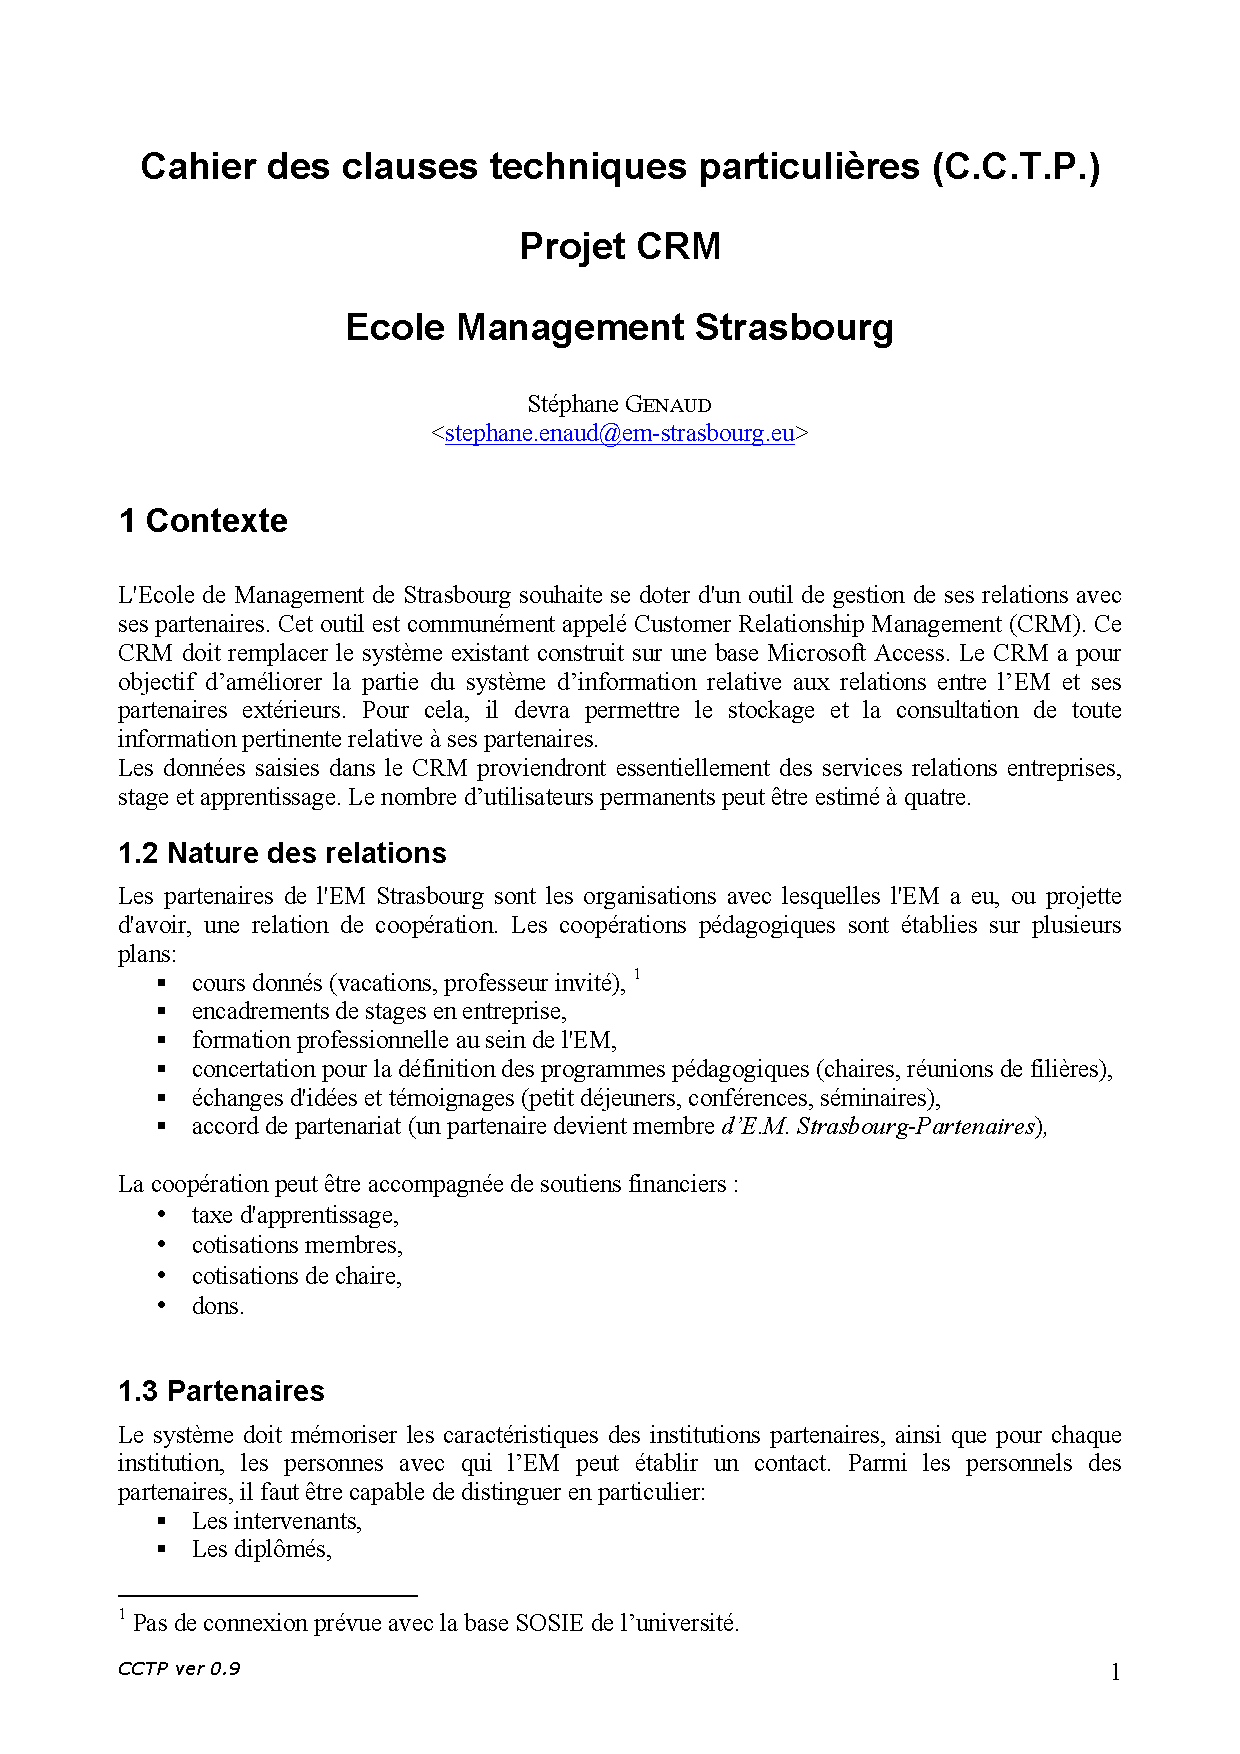
\includepdf[pages=1-5]{figs/crm_cctp.pdf}


\chapter{Base de données des CV}
\label{ch:rh-cvtheque}

Le document suivant décrit l'expression des besoins (dernière version du 9 mai 2011)
concernant le projet d'une base de donnée des CV.


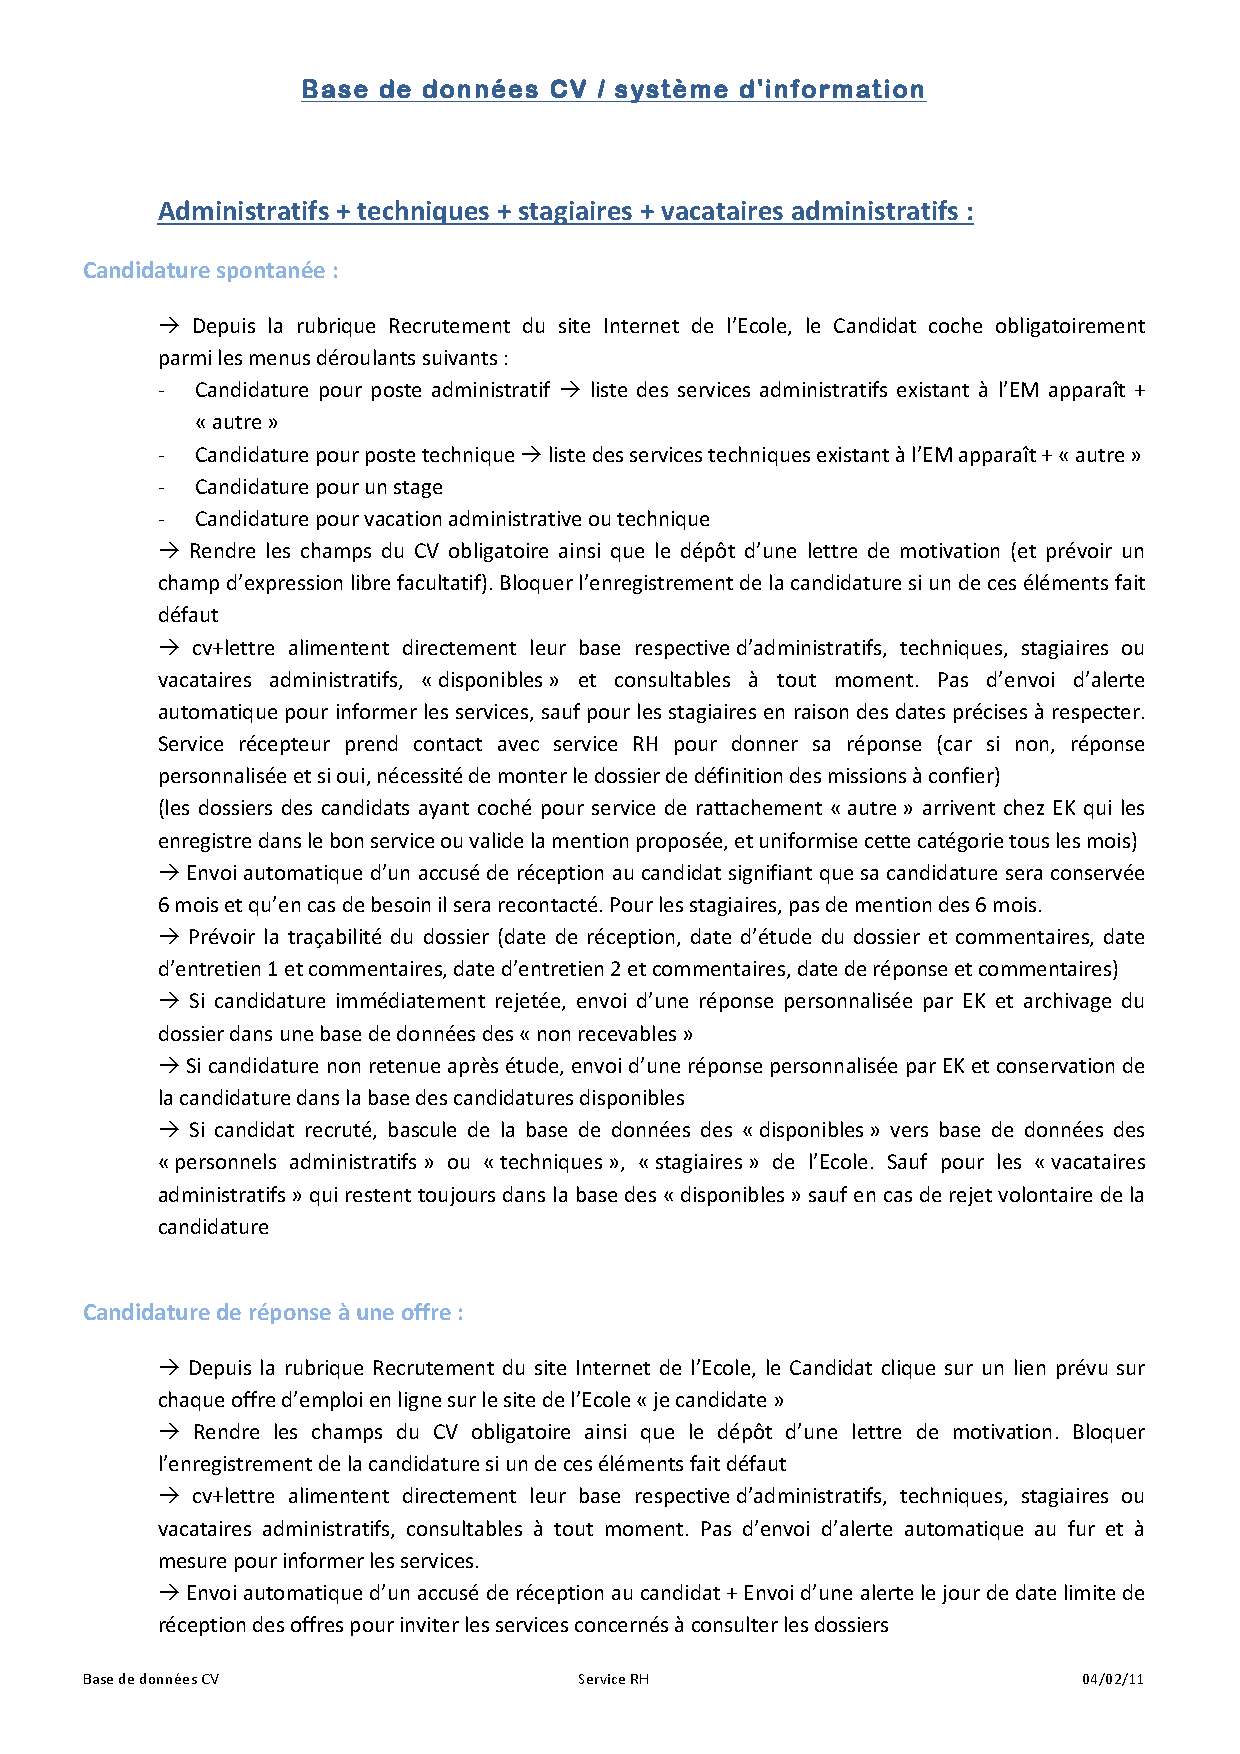
\includepdf[pages=1-4]{figs/rh-bdcv.pdf}

\end{document}

 
  
 

